%%%%%%%%%%%%%%%%%%%%%%%%%%%%%%%%%%%%%%%%%%%%%%%%%%%%%%%%%%%%%%%%%%%%%%%%%%%%%%%%%%%%%%%%%%%%%%%%%%%%%%%%%%%%%%%%%%%%%%%%%%%%%%%%%%%%%%%%%%%%%%%%%%%%%%%%%%%%%%%%%%%
% Written By Michael Brodskiy
% Class: Thermodynamics & Statistical Mechanics
% Professor: A. Stepanyants
%%%%%%%%%%%%%%%%%%%%%%%%%%%%%%%%%%%%%%%%%%%%%%%%%%%%%%%%%%%%%%%%%%%%%%%%%%%%%%%%%%%%%%%%%%%%%%%%%%%%%%%%%%%%%%%%%%%%%%%%%%%%%%%%%%%%%%%%%%%%%%%%%%%%%%%%%%%%%%%%%%%

\include{Includes.tex}

\title{Heat and Work}
\date{\today}
\author{Michael Brodskiy\\ \small Professor: A. Stepanyants}

\begin{document}

\maketitle

\begin{itemize}

  \item Heat ($Q$) and Work ($W$)

    \begin{itemize}

      \item $Q$ is the energy transferred \underline{to} $S$ through thermal contact with $R$

      \item $W$ is work done by/on $S$ through change in volume or external fields

    \end{itemize}

  \item \nth{1} Law of Thermodynamics

    $$\delta Q = dU+ \delta W$$

    \begin{itemize}

      \item $\delta$ is the inexact differential

      \item This means that:

        $$\oint df=0\text{ or }\int_1^2 df=\int_1^2 df$$

        \begin{itemize}

          \item $df$ is independent of path

        \end{itemize}

        $$\oint\partial f\neq0\text{ and }\int_1^2\partial f\text{ is path dependent}$$

      \item Note it \textit{may} equal 0, but does not have to

    \end{itemize}

  \item $U,\sigma$ are state functions, as they depend on state variables only ($\tau,V,N,\ldots$)

    \begin{itemize}

      \item $Q,W$ are not state functions (\textit{i}.\textit{e}.\ they are dependent on path)

    \end{itemize}

  \item Let us consider a reversible process — a process that does not increase the total entropy of $S+R$

    $$\delta Q_{rev}=\tau d\sigma$$

    \begin{itemize}

      \item In general:

        $$\delta Q\leq \tau d\sigma$$

      \item $Q$ is low quality energy; adding $\delta Q$ to $S$ increases its entropy by $\delta Q/\tau$

      \item $W$ is high quality energy

      \item Heat engines convert heat to work

        \begin{itemize}

          \item Steam engine
            
          \item Internal combustion

          \item Power plant

        \end{itemize}

    \end{itemize}

  \item Carnot efficiency $\eta_c$, is the ratio o work generate by $S$ to heat added to $S$ in a reversible process

    $$\eta_c=\left( \frac{W}{Q_h} \right)_{rev}$$

    \begin{itemize}

      \item This can be rewritten in many forms, including:

        $$\eta_c=\frac{Q_h-Q_l}{Q_h}=1-\frac{Q_l}{Q_h}=1-\frac{\tau_l}{\tau_h}$$

      \item The actual efficiency is:

        $$\eta\leq\eta_c$$

      \item This can be obtained by assuming $\sigma_h\leq\sigma_l$

    \end{itemize}

  \item Refrigerators use work to move heat

    \begin{itemize}

      \item The Carnot efficiency for a refrigerator is:

        $$\gamma_c=\left( \frac{Q_l}{W} \right)_{rev}$$

      \item This can be expressed in more useful terms for us as:

        $$\gamma_c=\frac{\tau_l}{\tau_h-\tau_l}$$

      \item Similar to heat engines, we can say:

        $$\gamma\leq\gamma_c$$

    \end{itemize}

  \item Carnot Cycle

    \begin{figure}[H]
      \centering
      \tikzset{every picture/.style={line width=0.75pt}} %set default line width to 0.75pt        

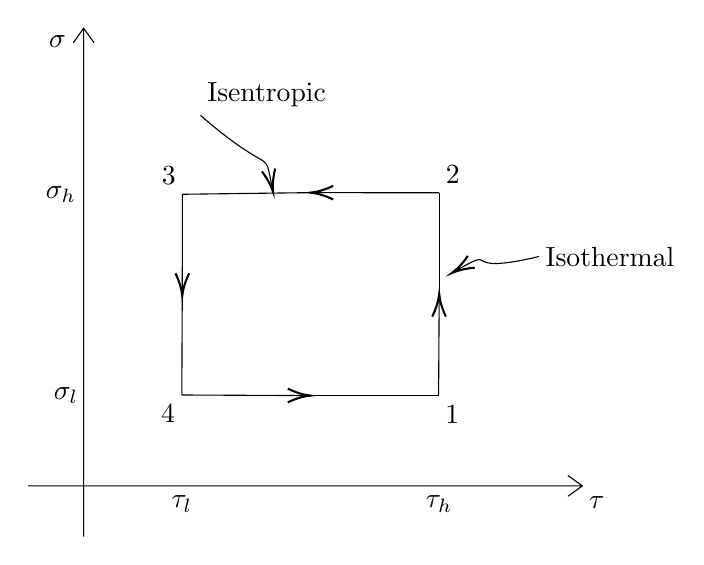
\begin{tikzpicture}[x=0.75pt,y=0.75pt,yscale=-1,xscale=1]
%uncomment if require: \path (0,444); %set diagram left start at 0, and has height of 444

%Shape: Axis 2D [id:dp10954316571485312] 
\draw  (187,247.5) -- (454,247.5)(213.7,27) -- (213.7,272) (447,242.5) -- (454,247.5) -- (447,252.5) (208.7,34) -- (213.7,27) -- (218.7,34)  ;
%Straight Lines [id:da7999053334568755] 
\draw    (384.71,204) -- (323,204) ;
%Straight Lines [id:da13773346411982845] 
\draw    (323,106.21) -- (261.29,107) ;
%Straight Lines [id:da8523825279579194] 
\draw    (261.21,156) -- (261,203.71) ;
%Straight Lines [id:da4522719625803868] 
\draw    (385,106.29) -- (385,155) ;
%Straight Lines [id:da29051283788172455] 
\draw    (261,203.71) -- (321,203.99) ;
\draw [shift={(323,204)}, rotate = 180.27] [color={rgb, 255:red, 0; green, 0; blue, 0 }  ][line width=0.75]    (10.93,-3.29) .. controls (6.95,-1.4) and (3.31,-0.3) .. (0,0) .. controls (3.31,0.3) and (6.95,1.4) .. (10.93,3.29)   ;
%Straight Lines [id:da018604575364712606] 
\draw    (385,106.29) -- (325,106.21) ;
\draw [shift={(323,106.21)}, rotate = 0.08] [color={rgb, 255:red, 0; green, 0; blue, 0 }  ][line width=0.75]    (10.93,-3.29) .. controls (6.95,-1.4) and (3.31,-0.3) .. (0,0) .. controls (3.31,0.3) and (6.95,1.4) .. (10.93,3.29)   ;
%Straight Lines [id:da43684644224945157] 
\draw    (384.71,204) -- (384.99,157) ;
\draw [shift={(385,155)}, rotate = 90.34] [color={rgb, 255:red, 0; green, 0; blue, 0 }  ][line width=0.75]    (10.93,-3.29) .. controls (6.95,-1.4) and (3.31,-0.3) .. (0,0) .. controls (3.31,0.3) and (6.95,1.4) .. (10.93,3.29)   ;
%Straight Lines [id:da05049902073104695] 
\draw    (261.29,107) -- (261.21,154) ;
\draw [shift={(261.21,156)}, rotate = 270.1] [color={rgb, 255:red, 0; green, 0; blue, 0 }  ][line width=0.75]    (10.93,-3.29) .. controls (6.95,-1.4) and (3.31,-0.3) .. (0,0) .. controls (3.31,0.3) and (6.95,1.4) .. (10.93,3.29)   ;
%Curve Lines [id:da7428626232053208] 
\draw    (433,137) .. controls (391.84,146.8) and (415.99,130.67) .. (392.5,144.14) ;
\draw [shift={(391,145)}, rotate = 330.02] [color={rgb, 255:red, 0; green, 0; blue, 0 }  ][line width=0.75]    (10.93,-3.29) .. controls (6.95,-1.4) and (3.31,-0.3) .. (0,0) .. controls (3.31,0.3) and (6.95,1.4) .. (10.93,3.29)   ;
%Curve Lines [id:da2554122965503123] 
\draw    (270,69) .. controls (306.08,100.2) and (300.32,82.92) .. (304.65,104.28) ;
\draw [shift={(305,106)}, rotate = 258.23] [color={rgb, 255:red, 0; green, 0; blue, 0 }  ][line width=0.75]    (10.93,-3.29) .. controls (6.95,-1.4) and (3.31,-0.3) .. (0,0) .. controls (3.31,0.3) and (6.95,1.4) .. (10.93,3.29)   ;

% Text Node
\draw (206.44,37.6) node [anchor=south east] [inner sep=0.75pt]    {$\sigma $};
% Text Node
\draw (456,251.4) node [anchor=north west][inner sep=0.75pt]    {$\tau $};
% Text Node
\draw (211.29,107) node [anchor=east] [inner sep=0.75pt]    {$\sigma _{h}$};
% Text Node
\draw (212.29,204) node [anchor=east] [inner sep=0.75pt]    {$\sigma _{l}$};
% Text Node
\draw (261,251.11) node [anchor=north] [inner sep=0.75pt]    {$\tau _{l}$};
% Text Node
\draw (385,251.11) node [anchor=north] [inner sep=0.75pt]    {$\tau _{h}$};
% Text Node
\draw (435,137) node [anchor=west] [inner sep=0.75pt]   [align=left] {Isothermal};
% Text Node
\draw (272,66) node [anchor=south west] [inner sep=0.75pt]   [align=left] {Isentropic};
% Text Node
\draw (386.71,207.4) node [anchor=north west][inner sep=0.75pt]    {$1$};
% Text Node
\draw (387,102.89) node [anchor=south west] [inner sep=0.75pt]    {$2$};
% Text Node
\draw (259.29,103.6) node [anchor=south east] [inner sep=0.75pt]    {$3$};
% Text Node
\draw (259,207.11) node [anchor=north east] [inner sep=0.75pt]    {$4$};


\end{tikzpicture}

      \caption{The Carnot Cycle}
      \label{fig:1}
    \end{figure}

    \begin{itemize}

      \item $1\to2$

        \begin{itemize}

          \item $Q_{12}=\tau_h(\sigma_h-\sigma_l)>0$

          \item $W_{12}=\tau_h(\sigma_h-\sigma_l)-(U_2-U_1)$

        \end{itemize}

      \item $2\to3$

        \begin{itemize}

          \item $Q_{23}=0$

          \item $W_{23}=-(U_3-U_2)$

        \end{itemize}

      \item $3\to4$

        \begin{itemize}

          \item $Q_{34}=\tau_l(\sigma_l-\sigma_h)<0$

          \item $W_{34}=\tau_l(\sigma_l-\sigma_h)-(U_4-U_3)$

        \end{itemize}

      \item $4\to1$

        \begin{itemize}

          \item $Q_{41}=0$

          \item $W_{41}=-(U_1-U_4)$

        \end{itemize}

      \item Total

        \begin{itemize}

          \item Work: $$(\tau_h-\tau_l)(\sigma_h-\sigma_l)>0$$

          \item Heat: $$(\tau_h-\tau_l)(\sigma_h-\sigma_l)>0$$

        \end{itemize}

      \item The efficiency may be defined as:

        $$\eta=\frac{W_{tot}}{Q_{rec}}=1-\frac{\tau_l}{\tau_h}$$

    \end{itemize}

  \item Subtle difference between isentropic and adiabatic (same if reversible): isentropic means constant entropy, adiabatic means no heat added to the system

  \item Carnot Cycle for an Ideal Gas (Spin 0, monatomic)

    \begin{figure}[H]
      \centering
      \tikzset{every picture/.style={line width=0.75pt}} %set default line width to 0.75pt        

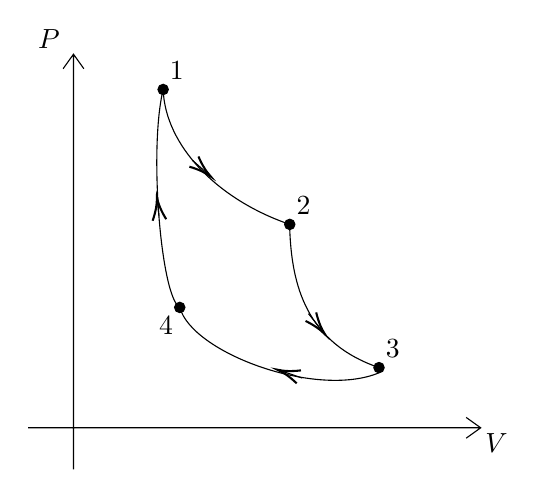
\begin{tikzpicture}[x=0.75pt,y=0.75pt,yscale=-1,xscale=1]
%uncomment if require: \path (0,444); %set diagram left start at 0, and has height of 444

%Shape: Axis 2D [id:dp246090509190372] 
\draw  (162,303) -- (380,303)(183.8,123) -- (183.8,323) (373,298) -- (380,303) -- (373,308) (178.8,130) -- (183.8,123) -- (188.8,130)  ;
%Curve Lines [id:da5468814941875568] 
\draw    (227,140) .. controls (228,167) and (253,193) .. (288,205) ;
%Straight Lines [id:da5595453548490974] 
\draw    (241,174) -- (248.51,180.67) ;
\draw [shift={(250,182)}, rotate = 221.63] [color={rgb, 255:red, 0; green, 0; blue, 0 }  ][line width=0.75]    (10.93,-3.29) .. controls (6.95,-1.4) and (3.31,-0.3) .. (0,0) .. controls (3.31,0.3) and (6.95,1.4) .. (10.93,3.29)   ;
%Shape: Circle [id:dp7297757219066234] 
\draw  [fill={rgb, 255:red, 0; green, 0; blue, 0 }  ,fill opacity=1 ] (290.5,205) .. controls (290.5,203.62) and (289.38,202.5) .. (288,202.5) .. controls (286.62,202.5) and (285.5,203.62) .. (285.5,205) .. controls (285.5,206.38) and (286.62,207.5) .. (288,207.5) .. controls (289.38,207.5) and (290.5,206.38) .. (290.5,205) -- cycle ;
%Curve Lines [id:da4015929743509441] 
\draw    (288,207.5) .. controls (289,234.5) and (296,262) .. (331,274) ;
%Straight Lines [id:da980202651862147] 
\draw    (297,248) -- (303.75,256.44) ;
\draw [shift={(305,258)}, rotate = 231.34] [color={rgb, 255:red, 0; green, 0; blue, 0 }  ][line width=0.75]    (10.93,-3.29) .. controls (6.95,-1.4) and (3.31,-0.3) .. (0,0) .. controls (3.31,0.3) and (6.95,1.4) .. (10.93,3.29)   ;
%Shape: Circle [id:dp5447799223437888] 
\draw  [fill={rgb, 255:red, 0; green, 0; blue, 0 }  ,fill opacity=1 ] (333.5,274) .. controls (333.5,272.62) and (332.38,271.5) .. (331,271.5) .. controls (329.62,271.5) and (328.5,272.62) .. (328.5,274) .. controls (328.5,275.38) and (329.62,276.5) .. (331,276.5) .. controls (332.38,276.5) and (333.5,275.38) .. (333.5,274) -- cycle ;
%Curve Lines [id:da06163707298536569] 
\draw    (331,276.5) .. controls (301,289) and (241,267) .. (235,245) ;
%Straight Lines [id:da7069468500369893] 
\draw    (294,279) -- (283.9,275.63) ;
\draw [shift={(282,275)}, rotate = 18.43] [color={rgb, 255:red, 0; green, 0; blue, 0 }  ][line width=0.75]    (10.93,-3.29) .. controls (6.95,-1.4) and (3.31,-0.3) .. (0,0) .. controls (3.31,0.3) and (6.95,1.4) .. (10.93,3.29)   ;
%Shape: Circle [id:dp9438557940404764] 
\draw  [fill={rgb, 255:red, 0; green, 0; blue, 0 }  ,fill opacity=1 ] (237.5,245) .. controls (237.5,243.62) and (236.38,242.5) .. (235,242.5) .. controls (233.62,242.5) and (232.5,243.62) .. (232.5,245) .. controls (232.5,246.38) and (233.62,247.5) .. (235,247.5) .. controls (236.38,247.5) and (237.5,246.38) .. (237.5,245) -- cycle ;
%Curve Lines [id:da12493331773667093] 
\draw    (235,245) .. controls (226,240) and (220,169) .. (227,140) ;
%Shape: Circle [id:dp4634916615897582] 
\draw  [fill={rgb, 255:red, 0; green, 0; blue, 0 }  ,fill opacity=1 ] (229.5,140) .. controls (229.5,138.62) and (228.38,137.5) .. (227,137.5) .. controls (225.62,137.5) and (224.5,138.62) .. (224.5,140) .. controls (224.5,141.38) and (225.62,142.5) .. (227,142.5) .. controls (228.38,142.5) and (229.5,141.38) .. (229.5,140) -- cycle ;
%Straight Lines [id:da1546077078212409] 
\draw    (225,201) -- (224.22,193.99) ;
\draw [shift={(224,192)}, rotate = 83.66] [color={rgb, 255:red, 0; green, 0; blue, 0 }  ][line width=0.75]    (10.93,-3.29) .. controls (6.95,-1.4) and (3.31,-0.3) .. (0,0) .. controls (3.31,0.3) and (6.95,1.4) .. (10.93,3.29)   ;

% Text Node
\draw (178.44,121.6) node [anchor=south east] [inner sep=0.75pt]    {$P$};
% Text Node
\draw (381,304.4) node [anchor=north west][inner sep=0.75pt]    {$V$};
% Text Node
\draw (229,136.6) node [anchor=south west] [inner sep=0.75pt]    {$1$};
% Text Node
\draw (290,201.6) node [anchor=south west] [inner sep=0.75pt]    {$2$};
% Text Node
\draw (333,270.6) node [anchor=south west] [inner sep=0.75pt]    {$3$};
% Text Node
\draw (233,248.4) node [anchor=north east] [inner sep=0.75pt]    {$4$};


\end{tikzpicture}

      \caption{$PV$ Diagram for Ideal Gas Carnot Cycle}
      \label{fig:2}
    \end{figure}

    \begin{itemize}

      \item Process $1\to2$ (Isothermal Expansion)

        \begin{itemize}

          \item $Q_{12}=\tau_h(\sigma_2-\sigma_1)=\tau_hN\ln\left( \frac{V_2}{V_1} \right)>0$

          \item $W_{12}=Q_{12}$ (from the $\delta Q=dU + \delta W$)

        \end{itemize}

      \item Process $2\to3$ (Isentropic/Adiabatic\footnote{Note; we may use either because the process is reversible} Expansion)

        \begin{itemize}

          \item $Q_{23}=0$

          \item $W_{23}=-\Delta U=-(U_3-U_2)=\frac{3N}{2}(\tau_h-\tau_l) >0$

        \end{itemize}

      \item Process $3\to4$ (Isothermal Contraction)

        \begin{itemize}

          \item $Q_{34}=\tau_lN\ln\left( \frac{V_4}{V_3} \right)=\tau_lN\ln\left( \frac{V_1}{V_2} \right)<0$

          \item $W_{34}=Q_{34}$

        \end{itemize}

      \item Process $4\to1$ (Isentropic Contraction)

        \begin{itemize}

          \item $Q_{41}=0$

          \item $W_{41}=-\Delta U=-\left( U_1-U_4 \right)-\frac{3N}{2}\left( \tau_l-\tau_h \right)<0$

        \end{itemize}

    \end{itemize}

  \item Work done by a reversible proess:

    $$\delta W=\tau\,d\sigma-dU$$

    \begin{itemize}

      \item Isothermal Process

        \begin{itemize}

            $$\delta W=-d(U-\tau\sigma)$$
            $$F=U-\tau\sigma$$

          \item This gives us:

            $$\delta W=-dF$$
            $$W=-\Delta F$$

          \item The work done by $S$ in a reversible, isothermal process is $-\Delta F$; $W<-\Delta F$ if the process is irreversible

          \item Thus, we can say the maximum work done by $S$ in any process at constant temperature is $\Delta F$

        \end{itemize}

      \item Isobaric Process

        \begin{itemize}

          \item The Work done by $S$ on the the environment is $P\,dV$, which is not very useful

          \item The effective work can be written:

            $$\delta W'=\tau\,d\sigma-dU-P\,dV$$

            \begin{itemize}

              \item Under constant temperature:

                $$\delta W'=-d\left( U+PV-\tau\sigma \right)$$

              \item We can introduce another quantity, $G$, the Gibbs free energy, such that:

                $$\delta W'=-dG$$
                $$W'=-\Delta G$$

              \item Similar statements for the Gibbs free energy can be made: $W_{eff}=-\Delta G$ for a reversible process, and $W_{eff}<-\Delta G$ for an irreversible process

              \item The enthalpy is $H=U+PV$

              \item Considering a case where $\delta W'=0$ (no effective work is done):

                $$\delta Q=d(U+PV)$$
                $$Q=\Delta H$$

            \end{itemize}

        \end{itemize}

    \end{itemize}

\end{itemize}

\end{document}



